\chapter{The solution}
\label{cha:main}
%\textit{Schema of the final solution, explanation of the flow and how it concretely works. Then, focus on three key components.}

\begin{figure}[H]
    \centering
    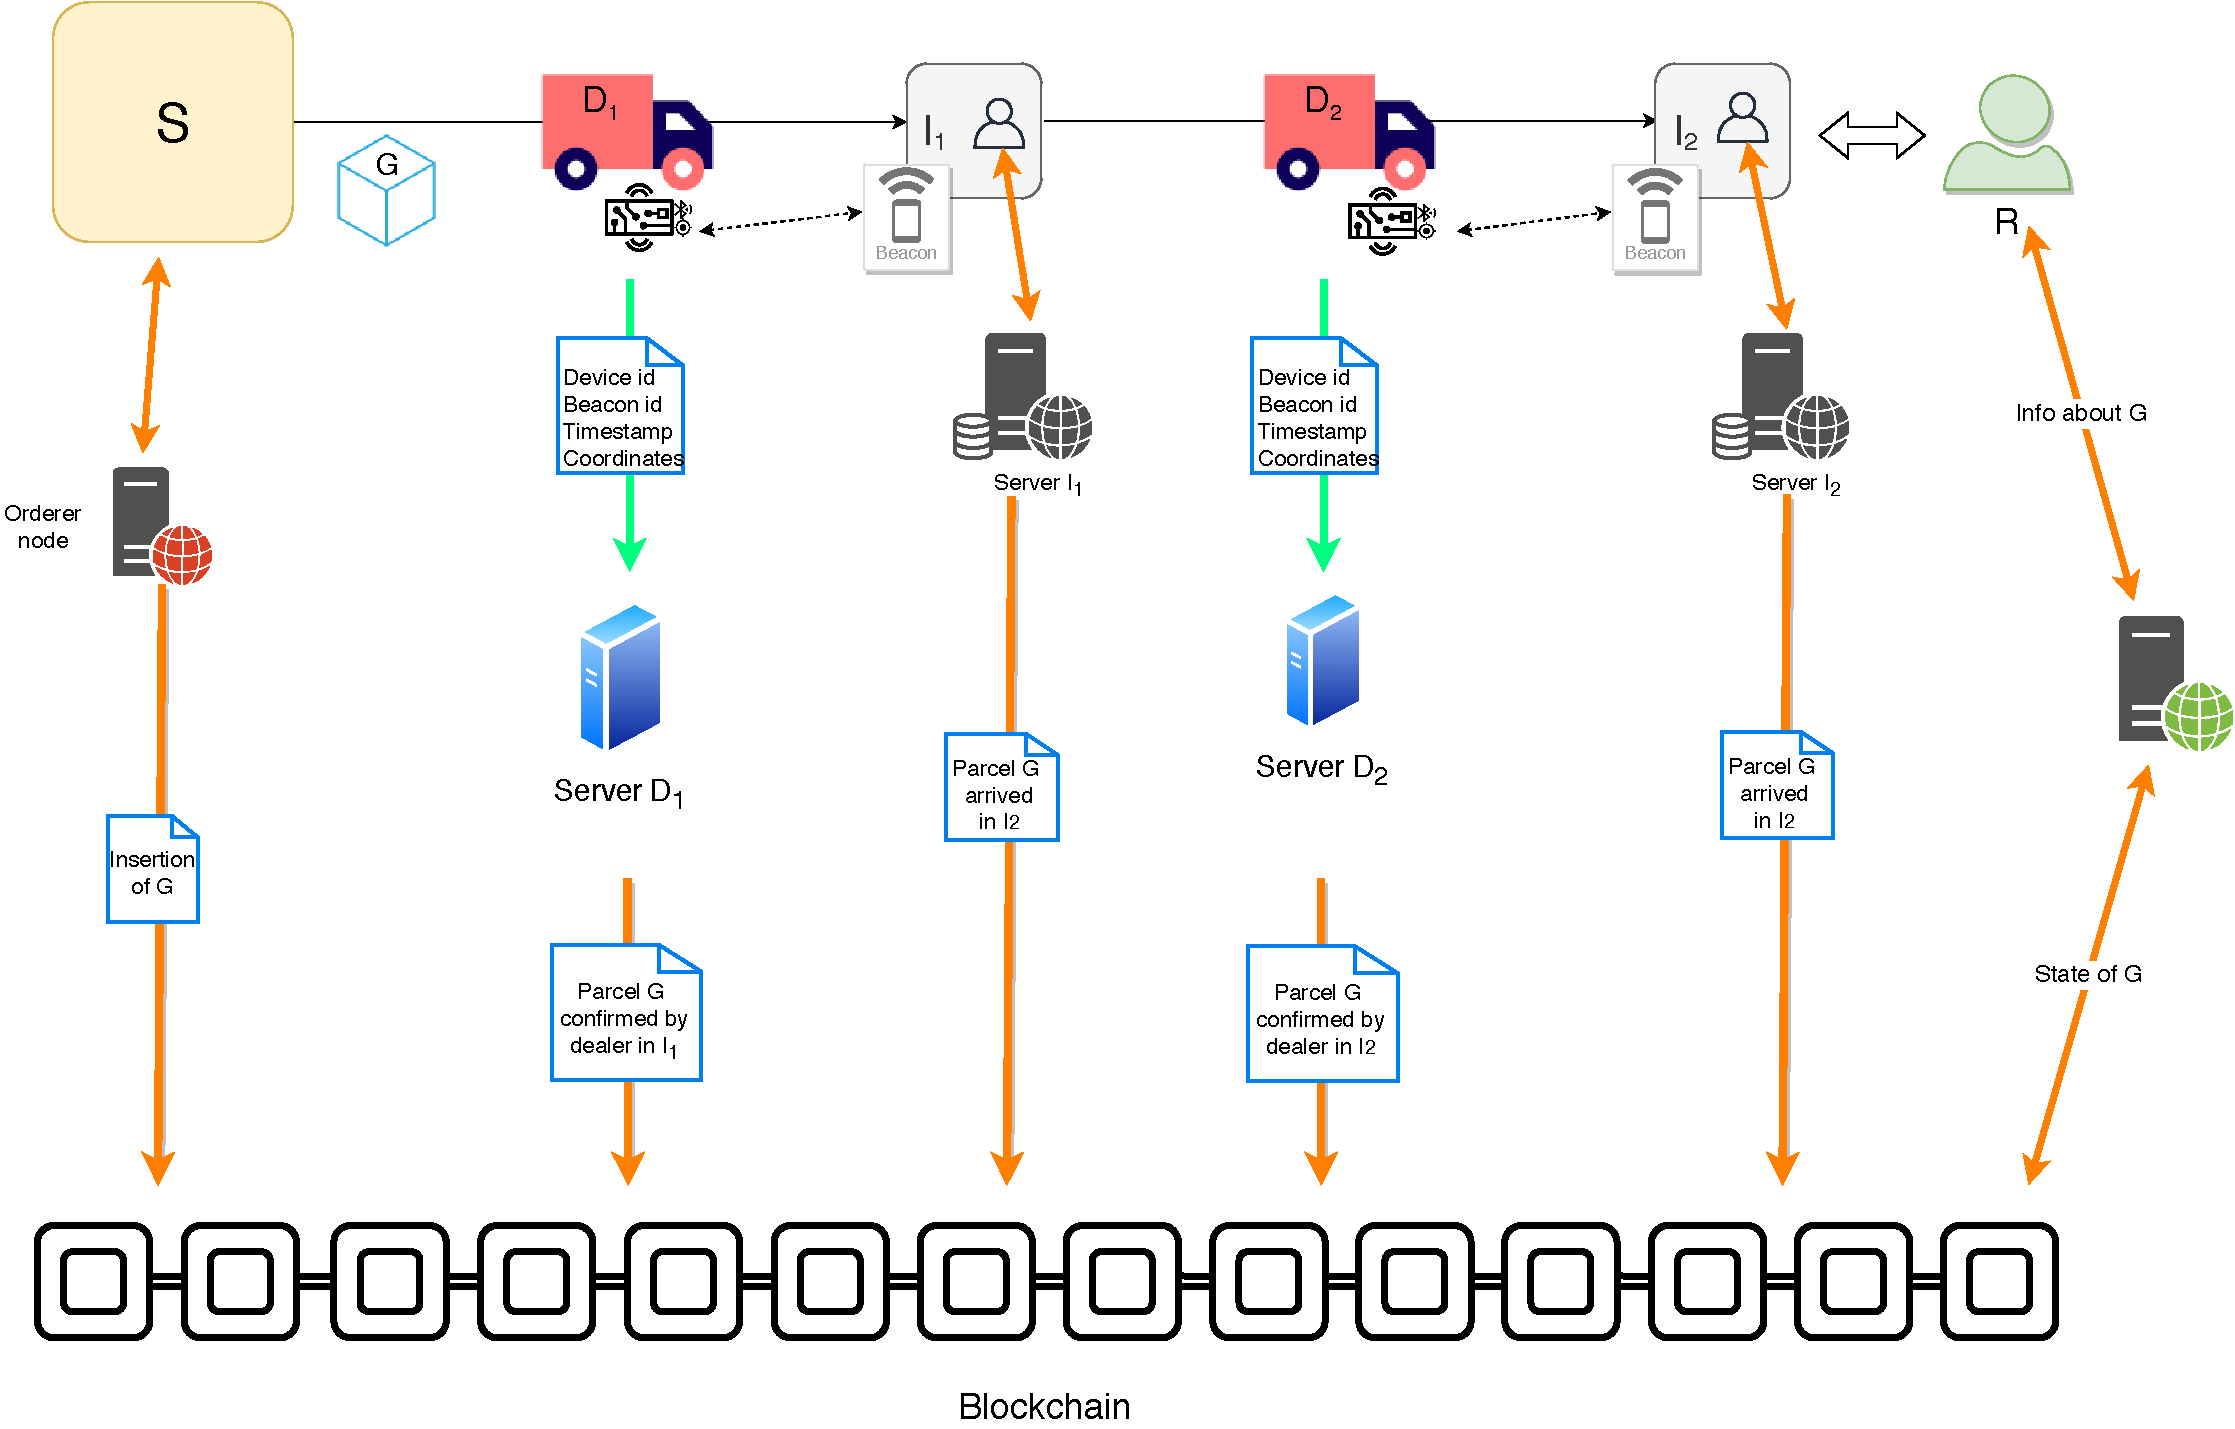
\includegraphics[scale=0.45]{figures/solution.pdf}
    \caption{The schema of the discussed solution}
    \label{fig:solution}
\end{figure}

Figure \ref{fig:solution} illustrates the solution that we have elaborated. Let us explain its characteristics, by first analyzing the overall flow and then concentrating in each step.

The notation used in the schema is the same as the one introduced in Chapter \ref{cha:background}: from left to right, we notice the sender \textit{S}, the good \textit{G}, two dealers $D_1$ and $D_2$, two intermediate points $I_1$ and $I_2$ (each one with a responsible person at work) and finally the receiver $R$. Obviously, this scenario is just a possible combination of entities and the solution is not fixed to this one.

The following is an abstract description of the various actions that are part of the model. For this moment we are ignoring some specific details (e.g. the protocols used for interactions, the format of the packets etc.), that will be properly explained together with the singular components.

$S$ starts the process by inserting into the system the information related to $G$. They have a dedicated server to provide the requested data. In particular, they need to declare the intermediate points and the dealers. This data will be stored in the blockchain as a new ``asset'', something similar to the coins in crypto-currencies. 

Then, the delivery is ready to start. $D_i$ (the procedure holds for both $D_1$ and $D_2$) carries an IoT device tracking its location and searching for other BLE devices nearby. On the other side, the intermediate stop has a beacon, constantly advertising its UUID (Universally Unique IDentifier). The protocol for the exchange is the following: 
\begin{itemize}
    \item The dealer arrives at the destination, the tracker detects the stop and sends to a server a packet containing the beacons' identifiers found;
    \item The server controls if one of the identifiers corresponds to the one owned by the intermediary and, if so, sends a confirmation to the blockchain;
    \item The person in control of $I_j$ collects $G$ and sends a confirmation, using a web interface, to a separate web server.
\end{itemize}

The model as it is so far cannot be deceived by the dealer, as they have no control over the device; however, it is vulnerable to an attack from a malicious actor controlling $I$. They can, in fact, collect $G$ and not inform the system about the exchange. As a result, we have lost track of who has the good. To solve this, there is the need for a protocol on the human side. Not complicated, but essential: the dealer has to make sure that who receives $G$ really sends their confirmation to the server. 

The final recipient, at any time, can access an interface that, by consulting the status of G on the blockchain, informs him about the progress of the delivery. They can check which exchanges happened and whether they succeeded. In case of problems it is immediate to find the responsible. Assuming that the protocol has been fully respected, if $G$ is only confirmed by the dealer it means that it is still in their hands; to the contrary, if only the intermediary confirmed the good, an error must have occurred, because there is no proof that the dealer really arrived at that place.

After this brief analysis there are a lot of unknown elements: how the devices work, how the communications take place, how the data is actually saved. In the next chapters we will discuss these aspects, dividing the project into the three main branches that constitute it.


\chapter{Tracking}
\label{sec:tracking}
%Introduction to what kind of tracking is needed, what we expect from the devices. Brief explanation of the state of the art of communication technologies (LoRa, SigFox, LTE, Wi-Fi, BLE, ...) and geolocalization.

The first part that we analyze is the tracking. Our solution needs devices that support geolocalization, bluetooth and can connect to the Internet to send messages. Clearly these are just the basic requirements, additional features can be useful in future developments. Another important aspect is the battery, since these devices cannot ensure long autonomy if frequently active. 

First, we will give a brief description of the modern technologies for the communications of IoT devices, then we will dive into the market to analyze the various options.

\section{Communication technologies}
\label{sec:track_comm}
%\textit{A brief analysis over the existing tracking technologies}

The state-of-the-art of these networks is very wide and presents several alternatives, each of them with advantages and disadvantages. They can be divided by many parameters, since many variables need to be taken into account when modelling the architecture of an IoT project. Our use case requires a standard able to guarantee the delivery of packets at arbitrary distance, consuming as little battery as possible. These requirements drive us to a new wireless communication techonology: LPWAN (Low Power Wide Area Network).

LPWAN is increasingly becoming popular thanks to its low-power, long-range and low-cost communication properties. It is particularly suitable for IoT applications that only need to transmit small amounts of data in long range and for its specifications it is preferable to traditional cellular options (such as 4G and LTE networks).

Many LPWAN technologies have been developed in both the licensed and unlicensed frequency bands. LoRa, Sigfox and NB-IoT are today the leading ones, with many technical differences \cite{LPWAN_study}.

\subsubsection{LoRa}
LoRa (Long Range) is a patented digital wireless communication technology that was first developed by Cycleo - a French start-up - and then acquired by Semtech (USA). Its ecosystem can be divided in two parts, LoRa and LoRaWAN: the latter is the standard protocol for WAN communications and the former is used as a wide area network technology. In other words, LoRa is the physical layer and LoRaWAN is the MAC and application layer of the stack.

LoRaWAN provides various classes of end devices to address different requirements. It ensures a better battery life compared to the other LPWAN technologies, but this also implies lower data rates and longer latency. To connect to the Internet, LoRa requires a gateway. The infrastructure is the following: end devices communicate with one or more LoRa gateways, which then forward messages to a cloud, a network server or to another gateway. On the contrary, when a message is sent to a device, the network chooses the best gateway.

One important aspect of LoRaWAN is determined by the so-called duty-cycle: defined as the maximum percentage of time during which an end-device can occupy a channel, is a key constraint for networks operating in unlicensed bands. Thus, each device has a threshold limiting the overall transmission time. However, the amount of time that a device will need is unknown, since it depends on the distance between the end point and the nearest gateway. The farther the gateway, the longer it will take to deliver a message. As a result, the total amount of messages sent is unknown and totally unpredictable considering our use case, in which we cannot make assumptions on the distribution of the gateways (w.r.t. the location of the tracker).

%To sum up: LoRaWAN is not proprietary and offers quite a good amount of flexibility, but it has some problems of coverage and infrastructure that does not make it the best choice.

\subsubsection{Sigfox}
Sigfox is a patented technology that was developed in 2010 by the start-up SigFox. It is an LPWAN network operator that uses a wide-reaching signal called ``ultra narrow-band''. This system presents a significant link asymmetry: a downlink communication, i.e., data from the base stations to the end devices can only occur following an uplink communication and in every case the number of messages is limited to 4 per day. On the uplink, instead, the amount of packets sent cannot be more than 140 per day, with a maximum payload length of 12 bytes. These limitations are similar to the LoRa's ones: in fact, they were included by the designers for the same reasons. Clearly, acknowledgements cannot be supported and consequently the reliability is ensured using time and frequency diversity as well as transmission duplication.

\subsubsection{NB-IoT}
NB-IoT is a radio technology standard developed by 3GPP (3rd Generation Partnership Project) to enable a wide range of cellular devices and services. It is based on the LTE protocol, therefore guaranteeing the high performance level associated with cellular connections, but at the cost of more complexity and greater power consumption. While other infrastructures have gateways that aggregate sensor data, which then communicate with the primary server, with NB-IoT sensor data is sent directly to it. For this reason it is being touted as the potentially less expensive option.

LTE-M is another LPWAN radio technology standard based on LTE. However, we did not take it into consideration because there is a lack of coverage and support from operators in Italy.

%We can conclude that, for our use case, the NB-IoT is the best alternative: despite the higher battery usage, it offers a solid and unrestricted network that can be used without creating a particular infrastructure or having to limit the number of messages.


\section{The market}
%\textit{The study and testing of the alternatives available, maybe a table summarizing the characteristics of each device (type of communication supported, battery, personalization of firmware, cost).}

The market of the IoT is constantly growing. There are numerous applications for these devices, both indoors and outdoors, with a variety of different requirements. For this reason, almost every company offers more than one solution, to best meet the needs of the buyer. We proceed now with the analysis of some candidate trackers. Table \ref{table_devices} summarizes their technical features.

\begin{table}[htbp]
\centering
\newcolumntype{Y}{>{\raggedright \arraybackslash}X}
\begin{tabularx}{\textwidth}{YYYYYY}
\toprule
\textbf{Company}        & \textbf{Device}         & \textbf{Connectivity}                                                          & \textbf{GNSS}                                & \textbf{Customizable firmware}           & \textbf{Additional}                                           \\ \midrule
Estimote       & LTE beacon     & Bluetooth 5.0, LTE-M/NB-IoT, NFC                                      & GPS, GALILEO, GLONASS               & No, but scripts can be included & accelerometer, temperature, LED, programmable button \\ \midrule
Accent Systems & IoT tracker    & Bluetooth 5.0, Wi-Fi, LTE-M/NB-IoT                                    & GPS, GLONASS, Galileo, QZSS, BeiDou & No                              & accelerometer, temperature, LED, buzzer              \\ \midrule
Sensolus       & Ultra          & BLE, Wi-Fi, Sigfox, GPS                                               & GPS                                 & No, but cloud API available     & accelerometer, temperature                           \\ \midrule
Pycom          & FiPy + PyTrack & Bluetooth, Wi-Fi, LTE-M/NB-IoT, LoRa, Sigfox & GPS, GLONASS, Galileo, QZSS         & Yes                             & accelerometer, LED                                   \\ \bottomrule
\end{tabularx}
\caption{Specifications of the devices}
\label{table_devices}
\end{table}

\subsubsection{Estimote, LTE beacon}
Estimote, Inc. \cite{estimote} is an American company that offers mostly beacons of different types. Their main focus is in indoor applications, but they also offer a device particularly close to our needs: the LTE beacon.

This tracker can connect to the Estimote cloud over LTE. Through this platform it is possible to include JavaScript code that will be run by the device, but the firmware itself is not customizable. This is the first negative point: every communication of the device is directed to its cloud and it is not possible to bypass it. Furthermore, the LTE beacon comes with a subscription including 1000 syncs per year per each device (for example, about 2-3 syncs per day). There’s also a data-cap of 100 MB per year.

%Even though the tracker offers a very good range of sensors and built-in radios, the limitations on the number of packets and the necessity to pass from its cloud make us definitely discard this candidate.
The tracker offers a good range of sensors and built-in radios. On the other hand, though, Estimote claims that, if frequently synced with the server, the battery life will be shorter than 2 days. Consequently, choosing the LTE beacon would imply the need of an external power bank or a permanent connection to the vehicle.

\subsubsection{Accent Systems, IoT tracker}
Accent Systems \cite{accentsys} designs and develops tailored IoT devices, offering an end-to-end solution. Like Estimote, they have a wide range of beacons and one particular device for outdoor tracking via LPWANs, called IoT tracker.

This solution is not personalizable in any way. The firmware is not modifiable and it communicates with a platform called Inmolecular (over LTE), a built-in ecosystem to show the tracker's data. The device, as specified in the website, is more destined to be integrated in an asset or in a vehicle to track only its location, not really to send custom packets as our project requires. Nevertheless, its characteristics make it a valid alternative.

\subsubsection{Sensolus, Ultra}
Sensolus \cite{sensolus} is an industrial IoT company, based in Belgium. Their main offer is addressed to logistic companies that want to track their assets. Indeed they propose an easy and ready-to-go service, similarly to the Accent Systems' one. Ultra is the tracker that we considered as a potential solution.

This is another device not open to personalization. However, the cloud exposes numerous APIs to read data sent by the trackers: the overhead is still present, but our server could coexist. Concerning the battery, the presence of a replaceable one is a double-edged sword, because on the one hand it is can ensure longer life, but on the other it requires an action to change it.

This device only supports Sigfox connectivity: the APIs are actually an extension of those provided by the operator. As pointed out in the previous section, this communication technology has some limitations in the number of messages that can be sent, which inevitably affect this tracker too.

\subsubsection{Pycom, Fipy and PyTrack}
Pycom \cite{pycom} offers hardware products that vary from plug and play devices to single components such as development boards and accessories. There are two separate products that together can form a good tracking solution: a development board (FiPy) and an additional module to support geolocalization (PyTrack).

This alternative is completely different from the other ones: instead of offering an entire environment, almost ready to use, this device comes completely empty and needs to be programmed. Even the battery is not present, so one can decide which one to use, or directly power it via cable. 

\section{The choice}
\label{sec:track_choice}
%\textit{Why we decided to choose that device: possibility to fully program the firmware, connectivity...}

Analyzing the various alternatives outlined we opted for the Pycom device. The first reason is the possibility of fully programming the firmware, which guarantees a high level of flexibility. Indeed, we need a complete control on the device: the algorithm needs to be elaborated and written by us. With all the other solutions, this would not possible; building our service on top of another one was not ideal.

In addition, the FiPy board offers a wide range of communication technologies that we could use: from the simple Wi-Fi for the developing phase to all the mentioned LPWANs. As for the latter, we identified NB-IoT the best technology. Similarly to the previous decision, we made this choice because, despite the higher battery consumption, it offers a solid, reliable and unrestricted network, which can be used without creating a particular infrastructure or having to limit the number of messages.

\section{Firmware}
\label{sec:track_firmware}
%\textit{Life cycle of the device (maybe with a flow chart). Some snippets?}

As aforementioned, the chosen device allow us to program its firmware completely. The programming language to be used is MicroPython \cite{micropy}, an implementation of Python 3 optimized for integrate controllers or constrained environments. It includes a subset of Python libraries, together with some modules specific to the MicroPython implementation.

The firmware is composed by two fundamental files: \texttt{boot.py} and \texttt{main.py}. When booting the device they are executed automatically. Usually the first is used to prepare the connectivity and perform the needed preliminary actions, while the second is the algorithm itself.

Figure \ref{flowchart} describes the device's life cycle. After booting, it attaches to the LTE network and initializes the Bluetooth and GPS sensors. Then, it tries to find the coordinates until it succeeds (actually, in the real implementation, a check is added, to handle cases in which it is impossible to locate the tracker; in other words, there is a maximum number of attempts). After the BLE scan, it checks whether the connection is still on: this is necessary because the dealer might have arrived in an area where there is no signal. Successively, it sends the data to the server, or it stores it in an internal file. Clearly, when the file is not empty and there is connection, the device will send the saved packets too. Finally, it turns off for a specific number of seconds, which is configurable.

% block styles
\tikzstyle{decision} = [diamond, draw, 
    text width=5.4em, text badly centered, node distance=3cm, inner sep=0pt]
\tikzstyle{block} = [rectangle, draw,
    text width=5em, text centered, minimum height=4em]
\tikzstyle{line} = [draw, -latex']
\tikzstyle{cloud} = [draw, ellipse,fill=red!20, node distance=3cm,
    minimum height=2em]
    
\begin{figure}[H]
\begin{tikzpicture}[node distance = 3cm, auto]
	% nodes
	\node [cloud] (start) {Start};
	\node [block, right of=start, yshift=-3em] (lte) {Attach to LTE};
	\node [block, right of=lte, xshift=1em] (initble) {Init Bluetooth};
	\node [block, right of=initble, xshift=1em] (initgnss) {Init GNSS};
	\node [block, below of=initble, yshift=-1em] (coord) {Search coordinates};
	\node [decision, right of=coord, xshift=1em] (foundcoord) {Coordinates found?};
	\node [block, below of=foundcoord, xshift=6em, yshift=-1em] (ble) {BLE scan};
	\node [decision, below of=ble] (conn) {Connected?};
	\node [block, left of=conn, xshift=-1em] (save) {Save to file};
	\node [block, right of=conn, xshift=1em] (send) {Send data};
	\node [block, below of=conn] (sleep) {Sleep for X minutes};
	% edges
	\path [line] (start) |- (lte);
	\path [line] (lte) -- (initble);
	\path [line] (initble) -- (initgnss);
	\path [line] (initgnss.south) -| ++(0pt, -15pt) -| (coord.north);
	\path [line] (coord) -- (foundcoord);
	\path [line] (foundcoord.south) |- node [near start] {no} ++(0pt,-20pt) -| (coord);
	\path [line] (foundcoord.east) -| node [near start] {yes} ++(20pt,0pt) -| (ble);
	\path [line] (ble) -- (conn);
	\path [line] (conn) -- node [near start] {yes} (send);
	\path [line] (conn) -- node [near start] {no} (save);
	\path [line] (save.south) |- ++(0pt, -20pt) |- (sleep);
	\path [line] (send.south) |- ++(0pt, -20pt) |- (sleep);
	\path [line] (sleep.south) -| ++(0pt, -15pt) -| (lte);
	
\end{tikzpicture}
\caption{Flowchart of the tracker's algorithm}
\label{flowchart}
\end{figure}

\chapter{Decentralized architecture}
\label{sec:arch}
%\textit{Requirements of the architecture, same as \ref{sec:tracking} (what we expect etc).}

After the individuation of the IoT devices, the second fundamental part of the project is the architecture. We already introduced in \ref{sec:decentralization} the intention of using a distributed network, possibly implementing a blockchain. However, there are different solutions that make use of this data structure to create a distributed ledger, that need to be analyzed. Unlike the previous sections, however, this time the decision will be more straightforward.

\section{Decentralization alternatives}
\label{sec:alternatives}
%\textit{Distributed databases, how they reach consensus, permissioned vs permissionless, blockchain based frameworks.}
There are two main alternatives for a blockchain-based architecture: permissionless and permissioned \cite{consensus_protocols}. In a permissionless blockchain, such as the cryptocurrencies ones, anyone can be a node of network, write in the shared ledger by proposing new transactions (that have to be validated) and participate in the process to reach consensus. In this scenario, the absence of trust is typically mitigated by introducing the ``mining'', a computational expensive process required to validate transactions. The term mining derives from the compensation given to the nodes that manage to approve a block, in form of transactions fees or new coins.

In contrast, permissioned blockchains are composed by known entities, which can be members of a consortium or stakeholders in a given business context; different methods are implemented to control and update the state, and there can be particular strategies to limit who can issue transactions. In this case, the risk of a malicious behaviour from a participant is considerably lower, because the guilty can be determined more easily. 

In our use case, the choice is simple: we have a precise set of participants that have a common goal, we want to make data available only to the nodes that need it and we do not plan to include a mining process. A permissioned blockchain is absolutely the best solution. Also concerning the framework, we did not consider many alternatives. There is one that perfectly suits our needs: Hyperledger Fabric. 

\section{Hyperledger}
\label{sec:hyperledger}
%\textit{Why (free and open source, easy to use, easy to install and deploy - mentioning Docker), description of what it is and how it works. Schema of our network using their notation.}
Hyperledger \cite{hyperledger} is ``an open source collaborative effort created to advance cross-industry blockchain technologies''. In other words, it is a group of related projects and tools, started by the Linux Foundation and supported by many IT companies (such as IBM and Intel), with the goal of offering blockchain-based solutions to build innovative applications. Under the Hyperledger ``umbrella'', there are several frameworks that range from permissionless to permissioned networks, with different targets. In particular, Fabric is the most interesting project for us: it offers a distributed ledger platform designed for industries, with a versatile and highly configurable architecture. It supports even pluggable consensus protocols and identity management protocols, enabling a full customization basing on the use case. Moreover, it is free, easy to use, install and deploy. Every peer of the network runs in Docker containers and the configuration of the network is made significantly simpler by tools like Composer and Explorer.

We have introduced a lot of elements that should be singularly explained. In the following sections we will describe accurately how Hyperledger Fabric works, how it is composed and how we built our network.

\section{Hyperledger Fabric structure}
\label{sec:fabric_structure}
In this section we will describe the main building blocks of Hyperledger Fabric.

\subsubsection{Assets}
Assets are the virtual coins exchanged in the Fabric environment. They can represent anything for which transactions are made. More specifically, they can be real products, like cars or houses, or intangible goods, like intellectual properties.

Concretely, assets are represented in the system as collections of key-value pairs, usually in JSON dictionaries. Every update of the assets is saved in the ledger.

In our system, as outlined previously, the assets are the goods being delivered. Their state is altered during the exchanges, through the submission of transactions, but the final recipient is always able to check every modification occurred.

\subsubsection{Smart contracts}
% in ETH transazioni scatenano contratti
% ETH non è una crypto, è blockchain
% fare capire che è un programma, Turing complete bla bla
Smart contracts are another concept related to a blockchain network: in general, they are self-executing scripts that are triggered by some conditions. For example Ethereum, another popular permissionless blockchain \cite{ethereum}, allows developers to program their ``autonomous agents'', using a particular DSL (Domain Specific Language), Solidity. This language is Turing-complete, so the smart contracts are concretely real programs, that can perform a wide range of actions. They can be used, for instance, so that funds are spent only when all the members of an organization (or a fixed percentage of them) give their authorization. 

In the Hyperledger environment, a smart contract defines the business logic that controls the lifecycle of the assets. It is also called ``chaincode'', interchangeably, even though the former is the transaction logic itself, while the latter is the container of a group of contracts which is then deployed in the network. 

In our use case, smart contracts are used to manipulate the state of the goods. The functions are executed on the ledger’s current state and are triggered by a transaction proposal. The result is a set of key-value pairs that can be applied to the ledger and distributed over all peers.

\subsubsection{Ledger}
Focusing now on the ledger itself, it can be described as the list of transactions maintained by each member of the network. It is composed by two parts. First, the ``chain'', which is the log of all transactions that have been made, kept in the tamper-resistant blockchain with all the properties outlined in \ref{sec:decentralization}. Second, the ``world state'', representing the latest values for all the keys. 

The current state is very important because it is the layer directly involved when transactions are submitted. To improve efficiency it is stored in a state database (such as LevelDB or CouchDB), which is basically an indexed view of the transaction log. It can always be regenerated from the chain.

The ledger contains also configuration blocks defining essential information such as access control lists and policies. We will explain better these concepts in \ref{sec:dev_tools}, to report how we used them.

\subsubsection{Peers}
Being one of the main reasons for which we chose this framework, the first characteristic of Fabric is that it is private and permissioned. The members of a network, indeed, have to enroll via an MSP (Membership Service Provider). This guarantees a complete control of the infrastructure and the possibility of identifying directly all the participants.

More precisely, each organization is responsible for setting up their peers. Each of them hosts an instance of the ledger and an instance of chaincode. As a result, redundancy is specifically introduced, to avoid single points of failure. Unlike public blockchains, though, the various peers have different roles, which we will list here. In the following section, a typical transaction flow will help understanding better how these roles come into play.

\begin{description}
    \item Orderer peers: the central nodes that group transactions in blocks and delivers them to all the other peers. They represent the direct source of consensus.
    \item Endorsing peers: the specialized peers designed to validate transactions. Fabric introduces them to increase scalability.
    \item Anchor peers: the discoverable peers that receive updates from the the orderers and broadcast them inside their organization.
    \item General peers: ordinary peers, that can submit transactions from their client applications. They basically act as proxies to connect clients to validating peers.
\end{description}

\textit{Missing: how the peers of our network represent these roles}

It can be pointed out that an orderer peer is potentially a single point of failure, thus exposing a Fabric network to the same problems of a traditional centralized architecture. If there is only one orderer node, this is true, but a real solution (in production) should consider this issue and avoid it. This point will be better clarified in the consensus section.

\subsubsection{Transactions}
We can summarize the typical Fabric workflow in six steps.

\begin{enumerate}
    \item A general node invokes a transaction request. This can be done through a client application.
    \item The general peer broadcasts the proposal to the required set of endorsing peers. How they are chosen depends on the endorsement policy defined for a chaincode, but intuitively it will be composed by the endorsing peers of each organization involved in that transaction proposal.
    \item Each of them checks the details needed to validate the transaction and runs the chaincode, independently. After that, they generate a response, containing the approval or the rejection of the proposal. 
    \item After receiving the needed number of positive responses, the peer sends the approved transaction to an orderer, to ensure that it is included in the ledger.
    \item Ordering nodes receive transactions from many different application clients concurrently. Their task is to work together to collectively form the ordering service, arranging batches of submitted transactions into a well-defined sequence and package them into blocks. After this, they have to forward the new block to the anchor nodes.
    \item Anchor nodes finally forward the block to the other peers inside their own organization. These individual peers then update their local ledger.
\end{enumerate}

\subsubsection{Consensus}
Consensus is a fundamental problem in distributed computing: in a nutshell, it consists in reaching an agreement among a collection of distributed processes.
As demonstrated by Fischer et al. \cite{consensus_impossible}, reaching consensus in a distributed system, under the hypothesis of faulty nodes and unreliable communications, is impossible. However, a good distributed system always exhibits stable intervals of correct functioning during which consensus is achieved, in practice. 

In Hyperledger Fabric the consensus problem is approached with the introduction of orderer nodes. Unlike permissionless blockchains, in which every node can participate in the consensus process and the algorithms involved guarantee consistency at a high probability, the ordering service ensures deterministic consensus. That is, in Ethereum or Bitcoin it is possible the generation of divergent ledgers, namely ``forks'', because the order of accepted transactions is not the same. A possible cause is the case of two (or more) miners forging different blocks at roughly the same time. These blockchains still have mechanisms to contrast this vulnerability, accepting only the longest chain and abandoning the so-called ``orphaned blocks''. However, the risk exists, while in Fabric once a block is generated it is guaranteed to be correct and final by design.

The documentation of Fabric presents several different implementations to achieve consensus in ordering service nodes. It is worth noting that no BFT (Byzantine Fault Tolerant) protocols are currently available, so the system is not capable of reaching agreement in the case of malicious nodes.
\begin{itemize}
    \item Solo, as the name suggests, features only one orderer node. Obviously, it is not fault tolerant, as it presents a centralized and vulnerable element. It cannot be a valid approach in production, but it can be useful when testing the architecture, because, from the other elements perspective, transactions are processed in the same way as with more complicated protocols. 
    \item Raft \cite{raft} is a CFT (Crash Fault Tolerant) protocol that has been introduced in v1.4.1. The underlying model includes a dynamically elected node which acts as a leader, that distributes its decisions among the others.
    \item Kafka \cite{kafka}
\end{itemize}
%\textit{How Hyperledger ensures consensus, reference to kafka and solo from the docs and the paper} 

\section{Development tools}
\label{sec:dev_tools}
%\textit{How we used them to build the network}
For the development phase, Hyperledger offers two powerful tools, that help modelling and testing an architecture before actually deploying it. Composer provides an abstract interface in which it is possible to create networks, while Explorer operates at a lower level and presents the REST APIs to query the blockchain or invoke transactions.

\subsection{Hyperledger Composer}
When building a new network it is advisable to start from this tool. The interface, called ``playground'', is very immediate and the documentation explains well how to use the various features offered. It is possible to use it directly in a web page, without installing anything, or loading the local version, that requires the development environment already set up. 

To deploy a business network in Composer there are some files that need to be created, in order to define the network properly.

\subsubsection{Model file}
The model file declares the various components of the network: the resources - namely participants, transactions, assets and events - and the support structures, such as enumerated types and concepts. We did not mention events previously, because they are concepts directly related to Composer; they can be emitted by the tool and subscribed to by external applications. They are triggered when a transaction is committed.

The file is written using an object oriented modeling language. Concretely, the resources are classes with fields that can be of primitive types or references to other classes. For transactions and events, identifiers and timestamps are automatically included. Our \texttt{model.cto} contains the definitions of four participants (the senders, the dealers, the intermediate points and the recipients), two transactions (confirmation from the dealer and confirmation from the intermediate point) and finally one asset (the good exchanged).

\subsubsection{Script file}
The script file is necessary to define the transaction logic for the business network. The functions created are executed when a transaction is submitted: referencing Section \ref{sec:fabric_structure}, it represents the chaincode.

A processor function is the logical operation related to a transaction defined in the model. It usually modifies one or more values contained in the assets and updates the registry. If required, it can emit an event. Unlike the model file however, the scripts are written in Javascript, a complete and powerful language that offers all its constructs to handle, for example, asynchronous code or external API calls.

In our project \texttt{script.js} simply implements the updates of the state of the asset when confirmations occur. Just a few checks are added to avoid the case of multiple confirmations from the same party and for the same good (which would be useless).

\subsubsection{Access control list}
This file defines the access control rules for business network. There are two types of access control: for resources and for network administrative changes. The evaluation follows a white list approach: if there is no rule granting a certain access, then it will be denied.

Each rule has to follow a precise grammar: it needs to have a description, a group or a particular participant (reported with the name inside the namespace), an operation (CREATE, READ, UPDATE, DELETE), a target resource (again using the namespace) and an action (ALLOW, DENY). Optionally, there can be conditions and transactions, defining the ones that the participant must have submitted in order to perform the specified operation.

In our network, the access control file (\texttt{permissions.acl}) is quite elaborated: we had to write a rule for participant to allow them to submit their transactions and to see the history of their operations only. Moreover, we denied the possibility of confirming a good from all the entities: even though this is a remote case, we do not want anyone but the participants directly involved to submit transactions about a certain delivery.

\subsubsection{Optional - Queries file}
This is a file with the purpose of defining some queries to retrieve information from the blockchain world-state. It is an optional component of the business network definition. 

All queries must contain the description and statement properties. The former is a simple string, which can be used to explain in human language the function of the query, the latter is the query itself. The statement is written in an SQL-like query language and can accept runtime parameters. In our project we did not include this file.
\vspace{11pt}

At this point we have all the elements that qualify a network. The model gives us the structure, the scripts are executed when transactions are submitted and everything is controlled by the access control rules. The missing part is how to actually test a network. Composer provides a test section, to create participants, assets and transitions. Everything is done ``behind the scenes'', by clicking on a graphic interface. On the one hand, this level abstraction is perfect to rapidly test the various files, but on the other there is the need to switch to a more concrete environment and test the real calls. That is why Hyperledger offers Explorer.

\subsection{Hyperledger Explorer}

\newpage
\chapter{Interfaces/Servers}
\textit{Small section with a bit of reference about the web servers and how they work. Some snippets can be useful here, explaining how we make use of the HyperLedger APIs. A little paragraph describing what MQTT is and why we decided to use it.}

